\documentclass[10pt, a4paper]{article}
\usepackage[spanish]{babel}
\usepackage[utf8]{inputenc}
\usepackage{graphicx}
\usepackage{multicol}
\usepackage[pdftex]{hyperref}
\usepackage{float}

\hypersetup{colorlinks,%
	    citecolor=black,%
	    filecolor=black,%
	    linkcolor=black,%
	    urlcolor=blue}

\begin{document}
    \begin{center}
    	\large Aprendizaje de M\'aquinas	\\
    	\huge \textbf{An\'alisis Grafol\'ogico} \\
    	
    	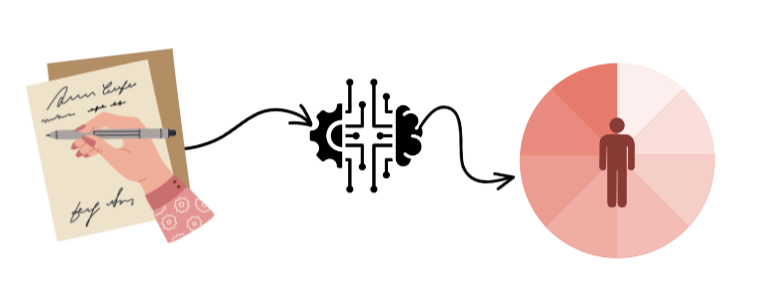
\includegraphics[height=5cm]{logo1.png}
    	
    	\normalsize Sheyla Leyva S\'anchez \\  Alejandra Monz\'on Pe\~na \\ Laura Victoria Riera P\'erez \\ Andry Rosquet Rodr\'iguez \\ Kevin Talavera D\'iaz \\ Javier Villar Alonso \\
    	
    	\vspace{1em}
    	\small Cuarto a\~no. Ciencias de la Computaci\'on. \\
   		\small Facultad de Matem\'atica y Computaci\'on, Universidad de La Habana, Cuba 
    \end{center}
	
	\vspace{0.05em}
	\normalsize
    \begin{abstract}
        La grafología es una técnica que estudia las características psicológicas de las personas a través de su escritura. 
        En algunos centros laborales se utilizan este tipo de análisis para determinar cuando contratar o no a alguien y se emplea también para analizar a criminales y en el proceso de determinar trastornos en personas. Esta es una tarea complicada realizada por expertos, psicólogos y grafólogos, y sus resultados están, numerosas veces, sujetos a la perspectiva de quien los analiza. 
        En este trabajo se propone utilizar algoritmos de Aprendizaje de Máquina, para automáticamente poder predecir características psicológicas de un individuo a partir de un fragmento de su escritura. 
        Con este objetivo se propone la creaci\'on de una base de datos de im\'agenes de escritura a mano, as\'i como su uso para entrenar y comparar los modelos para predecir la personalidad basado en el Test de los Cinco Grandes (Big Five).
        Se implementaron los algoritmos Convolutional Neural Network (CNN), Support Vector Machine (SVM), K-Nearest Neighbours (KNN) y K-Means, estableciendo una comparaci\'on de los resultados obtenidos para el an\'alisis grafol\'ogico. 
    \end{abstract}
    
    \section{Grafolog\'ia}
    
        La grafología es el análisis de la escritura manuscrita de un individuo con la intención de determinar rasgos de personalidad. 
        No existe evidencia científica que respalde la efectividad de la grafología, por lo que es considerada una pseudociencia 
        y una práctica científicamente cuestionable.\\ 

        Tal y como se menciona en el art\'iculo \cite{19} la grafolog\'ia no se utiliza para predecir el futuro o conocer el pasado de una persona. Su uso 
        est\'a dado como una habilidad para conocer el estado psicol\'ogico de la persona en el momento que escribe, incluso se plantea que los resultados de este an\'alisis 
        puede depender de la edad de la persona o del momento en que redacta; es decir una misma persona puede tener resultados diferentes si se analiza su escritura en dos momentos 
        diferentes de su vida.\\

        Según diversos estudios, si tienes un tamaño de letra grande es probable que seas una persona sociable, valiente y muy segura de ti misma. 
        Por otro lado, si tu letra es mediana, significa que te adaptas fácilmente a las circunstancias y eres abierto al cambio. 
        Por \'ultimo, si escribes con una letra de tamaño pequeño, tiendes a ser tímido, meticuloso e introvertido.\\

        Si el espacio que incluyes entre las letras es amplio, significa que aprecias tu libertad y que no te gusta sentirte abrumado o rodeado por mucha gente. 
        Si es angosto, no te agrada estar solo y prefieres vivir en compañía.\\

        En el art\'iculo \cite{17} analizan los rasgos de escritura con el objetivo de crear perfiles para los asesinos, en este art\'iculo explican que 
        rasgos psicol\'ogicos se vinculan a: Espaciado de palabras, Espaciado de l\'ineas, M\'argenes, Inclinaci\'on, Presi\'on del l\'apiz, Forma de letras i, Forma de letras t, entre otras. \\ 


    
    \section{Grafolog\'ia y Aprendizaje M\'aquina}
    
        La combinaci\'on de Aprendizaje M\'aquina y Grafolog\'ia es abordada en un amplio conjunto de art\'iculos en los que se prueban ideas diversas, e incluso se comparan los resultados obtenidos haciendo uso de
        diferentes t\'ecnicas y combin\'andolas.\\ 

        En los art\'iculos \cite{1} y \cite{2} abordan ideas de preprocesado de las im\'agenes manuscritas haciendo uso del umbral adaptativo Gaussiano y llevando a binario los valores de los p\'ixeles de la im\'agen atendiendo a un
        nivel de tolerancia prefijada.\\ 

        Las Redes Neuronales Convolucionales (CNN) debido a su amplio uso para el trabajo con im\'agenes, en el art\'iculo \cite{1} se usan las CNN como m\'etodo propuesto en la arquitectura de una p\'agina web que permita determinar la personalidad 
        a partir de la escritura. En otros como \cite{3} se emplea este m\'etodo en el an\'alisis de firmas, analizando la inclinaci\'on y el espaciado entre caracteres, con la limitaci\'on de que el dataset utilizado solamente posee 10 firmas de 6 individuos. \\ 

        De igual modo las CNN conjuntamente con Regresi\'on log\'istica se emplearon en \cite{4} para predecir el comportamiento financiero de una persona, en este caso con un dataset de más de 200 muestras de escrituras de un texto dado y resultados de un cuestionario de acuerdo al Big Five Personality Model.\\ 

        Otro algoritmo utilizado para el an\'alisis grafol\'ogico es SVM, empleado en \cite{2}, \cite{5}, \cite{6}, \cite{7} y \cite{8}. En el caso de \cite{6} emplean el algoritmo sobre firmas de 53 participantes, para obtener un 71\% de efectividad, 
        en otros como \cite{5} y \cite{8} se compara con otros algoritmos, en el primero con ANN y DNN y en el segundo con KNN y \'arboles de decisi\'on para predecir los resultados del Big Five, en este art\'iculo se utiliz\'o para el SVM un kernel RBF.\\ 

        Tambi\'en se utilizan: K-Means \cite{9}, Fuzy C-Means \cite{10}, ANN \cite{11,5,12,9}, Random Forest \cite{13, 14} y KNN \cite{14,9,8}.\\

        En el art\'iculo \cite{18} realizan un estado del arte sobre grafolog\'ia y Machine Learning en el cual comparan las investigaciones realizadas en 
        otros art\'iculos respecto a los Features utilizados, las caracter\'isticas del dataset, algoritmo empleado y resultados obtenidos.

    \section{Bases de Datos}

        Las bases de datos utilizadas en los estudios de grafolog\'ia realmente contienen informci\'on escasa. En muchos casos 
        son privadas y para acceder a ellas es necesario pagar. En el art\'iculo \cite{14} muestran una tabla comparativa de los datasets disponibles en 
        internet que se han utilizado en otros art\'iculos, en la misma describen cu\'ales son los tags presentes en cada uno de los datasets, si son p\'ublicos o no, en qu\'e atrt\'iculos se utilizan y 
        de que a\~no son. \\ 

        Al analizar este contenido resulta relevante que los tags que est\'an presentes en esos sets de datos son escasos, apenas ponen informaci\'on, como mano con la que escribe el sujeto, sexo, 
        ciudad en la que vive y poco m\'as. \\ 

        Se descargaron los datasets de HandwritingDatabase \cite{15} y iam-handwriting-database \cite{16}, el primero conten\'ia un conjunto de im\'agenes de textos manuscritos e informaci\'on de cada persona como sexo, estado de EEUU donde naci\'o 
        mano con la que escribe y edad, el segundo conten\'ia las im\'agenes de textos, las mismas segmentadas por l\'inea, por palabra y por caracteres y ten\'ia informci\'on general sobre los textos como 
        ancho de l\'inea, altura de l\'inea, cantidad de palabras por l\'inea, etc; pero ninguna informaci\'on sobre las personas. \\ 

        Debido a la dificultad de descargar un dataset y la poca informaci\'on que ofrecen los datasets disponibles para el problema que deseamos resolver, se decidi\'o elaborar una base de datos propia.

    \section{Creaci\'on de la Base de Datos}

        La propuesta es crear nuestro propio dataset, para ello fueron encuestadas 71 personas, a las que se les pidi\'o que escribiesen un texto 
        en espa\~nol y se les realiz\'o el test de personalidad BigFive \cite{23}. \\ 

        Las hojas manuscritas fueron escaneadas y a las im\'agenes se les aplic\'o un preprocesado para llevarlas escala de grises y finalmente a binario con un nivel de tolerancia de 180. Adem\'as se 
        realiz\'o una segmentaci\'on de los textos en l\'ineas a partir de una difusi\'on de los caracteres utilizando \texttt{opencv} de python. Las secciones de imagen que no quedaran 
        del todo segmentadas producto a escrituras muy unidas fueron segmentadas manualmente.\\ 

        A los test de personalidad se les extrajo autom\'aticamente la informaci\'on referida a los porcentajes de cada uno 
        de los 5 rasgos distintivos del Big Five, para esto se emple\'o un c\'odigo de python que scrapea las p\'aginas web de los resultados del test.\\ 

    \section{Extracci\'on de Features}
        Para extraer los features de las im\'agenes del DataSet se utilizaron algoritmos de procesamiento de im\'agenes. Previamente a las im\'agenes se les realiz\'o un 
        preprocesado para eliminar ruidos y llevarlas a binario; los features extra\'idos son: Interlineado (LineSpace), Espaciado (WordSpace), Margen (Margin), Inclionaci\'on de la l\'inea (Baseline) e Inclinaci\'on de las letras (Slant). 

        \subsection{Interlineado} 

            Para el interlineado se analizan dos clasificaciones posibles: Interlineado amplio (LINESPACE\_SEPARETED) e Interlineado peque\~no (LINESPACE\_CROWDED). Para encontrar el interlineado se utiliz\'o la t\'ecnica del perfil 
            de proyeci\'on vertical suavizado(SPR) \cite{20}, esto permite separar las zonas de texto y espacios analizando los extremos del SPR, para las im\'agenes segmentadas es simple con este algoritmo determinar donde est\'a el texto correspondiente a la l\'inea y los espacios superior e inferior
            correspondientes al interlineado, as\'i se puede determinar si una l\'inea est\'a muy unida a sus adyacentes considerando la proporci\'on de p\'ixeles de foreground (p\'ixeles negros correspondientes a texto) que existen en 
            las regiones identificadas como espacio. \\

            Para analizar los SPR se separa la imagen en regiones verticales de tama\~no 5\% del ancho de la imagen. Luego, se hace el SPR de cada uno, se determinan las regiones de texto y espacio \cite{22} y se calcula la densidad 
            de p\'ixeles de foreground en los espacios. Finalmente, se promedian los resultados de densidades para cada secci\'on vertical, para determinar si la l\'inea est\'a muy separada o muy pegada a sus adyacentes. 

            \begin{figure}[H]
                \centering
                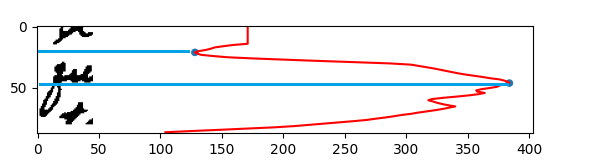
\includegraphics[width = 0.5\linewidth]{Figure_1.png}
                \caption{Segmento vertical de 5\% de imagen, en rojo el SPR y en azul los extremos del SPR, en el intermedio est\'a la zona de texto y en los bordes la zona de interlineado.}
            \end{figure}
        \subsection{Margen} 
        
            Para determinar el margen se pueden considerar tanto los m\'argenes superior e inferior como los m\'argenes laterales \cite{21}. Para nuestro Dataset, como las im\'agenes son l\'ineas manuscritas, no tiene sentido analizar los m\'argenes superior e inferior. Por tanto, solo 
            se clasifica el margen lateral izquierdo en cuanto a su ancho como: Margen ancho (BIG\_MARGIN) y margen estrecho (SMALL\_MARGIN). Para esto se analiz\'o el perfil de proyeccci\'on (PR) horizontal de cada im\'agen tomando el rango del PR desde el elemento 0 hasta que el valor del PR 
            sea mayor que una tolerancia especificada; es decir, mientras que la densidad de p\'ixeles en el foreground para cada columna de la imagen sea menor que un valor relativo al largo de la imagen. 

            \begin{figure}[H]
                \centering
                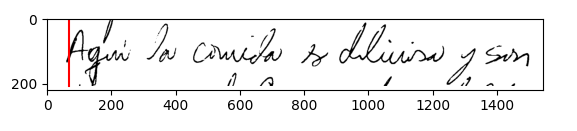
\includegraphics[width = 0.5\linewidth]{Margin.png}
                \caption{Desde el inicio hasta la l\'inea roja la secci\'on de margen.}
            \end{figure}
        \subsection{Espaciado} 

            El espaciado, son los espacios dejados entre caracteres y palabras en una misma l\'inea. Para clasificar el espaciado se realiz\'o a cada imagen un trabajo con filtros morfol\'ogicos; seleccionando un kernel horizontal para realizar una convoluci\'on con la imagen 
            que permita unificar los trazos de todo lo que est\'e escrito unido de una misma palabra para de este modo separar las palabras enmarc\'andolas en recuadros. As\'i el espaciado se puede determinar como la distancia promedio entre los recuadros.

            \begin{figure}[H]
                \centering
                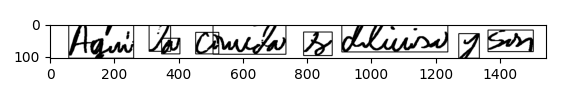
\includegraphics[width = 0.5\linewidth]{Espaces.png}
                \caption{Recuadros que bordean al texto escrito sin espacios.}
            \end{figure}

        \subsection{Inclinaci\'on de la L\'inea}
            Para determinar la inclinaci\'on de la letra en una l\'inea se realiz\'o el procedimiento descrito en \cite{20}, rotando la im\'agen desde $-30^{\circ}$ hasta $30^{\circ}$. 
            Determinando para cu\'al de los valores de la rotaci\'on la cantidad de p\'ixeles de foreground es m\'axima para la zona central de la imagen. Para los \'angulos comprendidos 
            entre $ [-30; -5) $ se dice que la linea base es Ascendente (ASCENDING), entre $[-5; 5]$ es Nivelada (LEVELED) y entre $(5; 30]$ es Descendente (DESCENDING). 

            \begin{figure}[H]
                \centering
                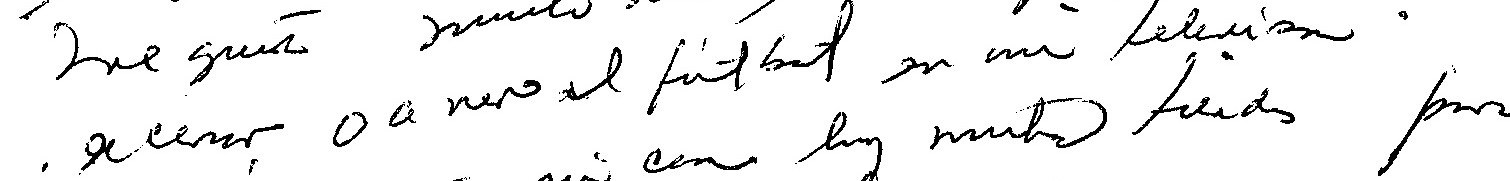
\includegraphics[width = 0.4\linewidth]{Judith_21.jpg}
                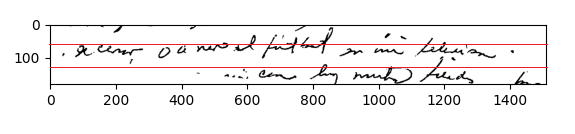
\includegraphics[width = 0.4\linewidth]{Baseline.png}
                \caption{a) texto original b) Texto con una inclinaci\'on de $-6^{\circ}$, la zona enmarcada en rojo es el \'area en que se busca maximizar 
                la cantidad de pixeles de foreground.}
            \end{figure}

        \subsection{Inclinaci\'on de la letra}
            Para la inclinaci\'on de la letra se tienen 5 posibles clasificaciones: Inclinado extremadamente a la izquierda (EXTREME\_LEFT), ligeramente inclinado a la 
            izquierda (MODERATE\_LEFT), as\'i como sus equivalentes hacia la derecha (EXTREME\_RIGHT) y (MODERATE\_RIGHT) respectivamente y la escritura sin inclinaciones (VERTICAL). 
            Para extraer este feature se utiliza el perfil de proyecci\'on (PR) vertical rotando la imagen en \'angulos entre $-20^{\circ}$ y $20^{\circ}$, buscando el \'angulo que maximice
            la suma del PR normalizado, tal y como se plantea en \cite{20}.

    \section{Algoritmos Utilizados}
        Para la investigsci\'on sobre Grafolog\'ia con aprendizaje de m\'aquinas se utilizaron a modo comparativo los algoritmos m\'as citados en el Estado del Arte de este tema. 
        Para probar cada uno de ellos se dividi\'o el dataset en  conjuntos: Entrenamiento/Test y Validaci\'on con tama\~no $75\%$ y $25\%$ de las personas que conforman el dataset respectivamente.
        Primero se seleccion\'o el conjunto de personas para hacer la validaci\'on y se separaron las im\'agenes de sus escrituras, features extra\'idos y resultados del test BigFive. Luego a los restantes datos del dataset 
        se les aplic\'o k-fold para dividir los datos de tests y entrenamiento.  
        
        \subsection{KNN}
            Para el algoritmo de KNN se utilizaron los features extra\'idos de las im\'agenes y los resultados del big five para entrenar un modelo \texttt{KNeighborsClassifier} del m\'odulo sklearn de pyrhon. 
            Previo al entrenamiento se reescalaron los datos de la entrada utilizando \texttt{StandardScaler}. El valor de k fijado como cantidad de vecinos cercanos a fijar fue 7, con el cual se obtuvo los mejores resultados en 
            la etapa de entrenamiento/test del algoritmo previo a la validaci\'on final. Cada caracter\'istica se predijo por separado y se emple\'o una agrupaci\'on en intervalos de a 10.
        
        \subsection{CNN}
            En la Red Neuronal Convolucional se utiliz\'o directamente las matrices de pixeles de las im\'agenes de escrituras para entrenar el modelo. 
            Primeramente se hizo un reescalado de la imagen para que todas tuviesen la misma resoluci\'on y luego se utilizaron en el entrenamiento de una CNN.
            Para la \'ultima capa de la CNN se tienen 5 neuronas, una por cada uno de los rasgos del BigFive a predecir.\\
            
            Se probaron con varias ideas de entrenamiento, variando las dimensiones de las im\'agenes para determinar si la calidad afecta en mayor o menor medida la clasificaci\'on. No obstante teniendo en cuanta las caracter\'isticas del dataset, en cuanto al vol\'umen de im\'agenes el modelo con Redes Neuronales es propenso 
            a overfit con pocas im\'agenes. 
        
        \subsection{SVM}
            Para la m\'aquina de soporte vectorial, como las clasificaciones seg\'un BigFive para cada uno de los rasgos punt\'ua con un valor de 0 a 120, y SVM separa por categor\'ia,
            reescalamos los resultados deo BigFive de 0 a 11, agrupando los valores del big five de 10 en 10. Como adem\'as los rasgos del Big Five son independientes, si con la grafolog\'ia fuera posible determinarlos, su valor depender\'ia solo de los rasgos de las letrasy no uno de otro.
            Por tanto se cre\'o una SVM por cada uno de los 5 rasgos de Big Five de modo que permita clasificar para cada persona los niveles de cada caracter\'istica en que se encuentra. Para esto se enten\'o el modelo \texttt{SVC} de sklearn.svm con los features extra\'idos de las fotos y con uno de los rasgos del BgFive en cada caso.
            Los datos fueron reescalados usando \texttt{StandardScaler} de sklearn.preprocessing.
            Como la clasificaci\'on es de m\'as de 2 categor\'ias se emple\'o una estrategia de clasificaci\'on de one-versus-one (ovo) y se prob\'o el enfoque con los kernels: lineal, polinomial y rbf. De igual modo se hizo un an\'alisis seprando los rasgos en solo 2 categorias, Alto (1) y Bajo (0) y un an\'alisis final intentando predecir 
            los 5 rasgos en simult\'aneo
			
       \subsection{K-Means}
			Se utiliz\'o el modelo \texttt{KMeans} de sklearn.clusters con los datos procedentes de los features extra\'idos de las im\'agenes y los resultados del test BigFive, siguiendo dos enfoques para el an\'alisis: a partir de los features determinar las caracter\'isticas de la personalidad asociadas; y viceversa, a partir de los resultados del big five tratar de hallar los rasgos de la escritura que se repiten a trav\'es de los cl\'usters. Para determinar el n\'umero de cl\'usters K que mejor se ajusta a los datos se implementaron el m\'etodo del codo para las medidas de inercia y distorsi\'on, y el m\'etodo de la silueta. Adem\'as se implementaron m\'etodos para poder visualizar todos estos resultados en distintas dimensiones. 
			
    \section{Resultados}
            \subsection{KNN}
                En la evaluaci\'on del KNN se tuvieron en cuenta las m\'etricas de \texttt{acurracy} y \texttt{precision}. Para cada uno de los rasgos por separado se
                obtuvo en la etapa de entrenamiento/test los sigientes valores promedio para esas m\'etricas luego de utilizar un 5-Fold: \\

                \begin{tabular}[H]{|c|c|c|}

                    \hline Categor\'ia & Accuracy promedio & Precisi\'on promedio \\  
                    \hline Neuroticismo & 0.543033653236376 & 0.43342082642200563 \\
                    \hline Extroversio\'n& 0.5431921954931721 & 0.5473437650759438 \\
                    \hline Apertura a Experiencias & 0.41551811609520994 & 0.43320995174546806 \\
                    \hline Simpat\'ia& 0.8458440789751829 & 0.42945218290696635 \\
                    \hline Moralidad & 0.7041812877859046 & 0.5274896102039315 \\
                    \hline
                \end{tabular}

                \begin{figure}[H]
                    \centering
                    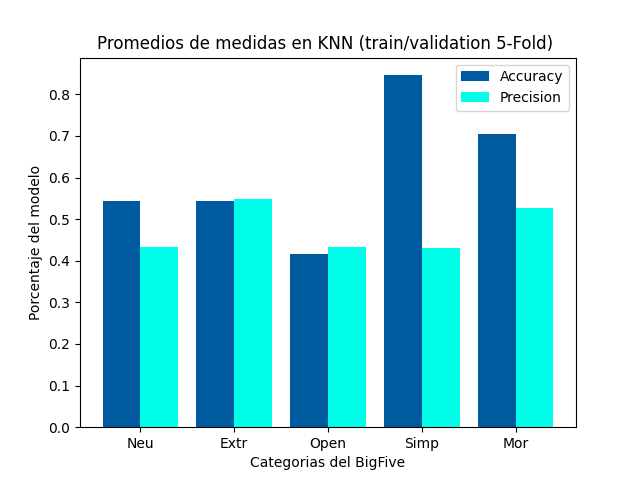
\includegraphics[width = 0.7\linewidth]{bar_knn.png}
                \end{figure}

                Posteriormente en la etapa de validaci\'on los resultados que se obtienen para \texttt{acurracy} y \texttt{precision} de cada rasgo son: 

                \begin{tabular}[H]{|c|c|c|}
                    \hline Categor\'ia & Accuracy & Precisi\'on \\  
                    \hline Neuroticismo             & 0.910828025477707  & 0.4798657718120805 \\
                    \hline Extroversio\'n           & 0.4681528662420382 & 0.37875375375375375 \\
                    \hline Apertura a Experiencias  & 0.2611464968152866 & 0.5211134453781512 \\
                    \hline Simpat\'ia               & 0.8885350318471338 & 0.45737704918032784 \\
                    \hline Moralidad                & 0.9140127388535032 & 0.46141479099678456 \\
                    \hline
                \end{tabular}
            
                \begin{figure}[H]
                    \centering
                    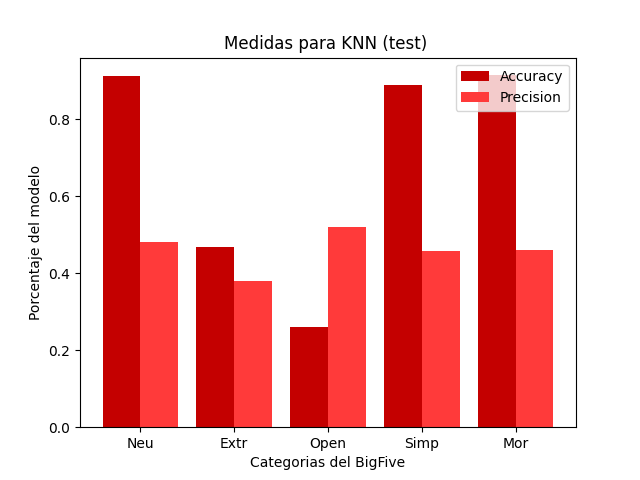
\includegraphics[width = 0.7\linewidth]{bar2_knn.png}
                \end{figure}

            \subsection{CNN} 
                Para la Red Neuronal Convolucional se analizaron los rasgos del BigFive agrupando los valores de cada caracter\'istica en rangos de a 10. 
                Se tuvieron en cuenta para la evaluaci\'on del modelo las m\'etricas: \texttt{mean absolute error} (MAE) y el \texttt{accuracy}.
                Los resultados para cada tama\~no de entrada obtenidos son los siguientes: \\

                Usando 3 capas de convolucion, reajuste de las im\'agenes a 32x32:\\
                \begin{itemize}
                    \item[] MAE para caracter\'istica 0: 1.3867782231034904 
                    \item[] MAE para caracter\'istica 1: 1.304610701813095 
                    \item[] MAE para caracter\'istica 2: 0.9960057525342452
                    \item[] MAE para caracter\'istica 3: 1.356362326391812
                    \item[] MAE para caracter\'istica 4: 1.3710135627980433
                \end{itemize}
                
                Con un accuracy igual a 76.048\%.\\

                Si se entrena con exactamente las mismas caracter\'isticas pero con im\'agenes ajustadas a 64x64, para mayor calidad, obtenemos los siguientes resultados:
                \begin{itemize}
                    \item[] MAE para caracter\'istica 0: 1.2410950697244811
                    \item[] MAE para caracter\'istica 1: 1.0932612272971434
                    \item[] MAE para caracter\'istica 2: 0.9566778752995634
                    \item[] MAE para caracter\'istica 3: 1.0583139525519476
                    \item[] MAE para caracter\'istica 4: 1.2694159266592442
                \end{itemize}
                
                Con un accuracy igual a 75.901\%.\\

                Haci\'endolo con dimensiones 128x128:
                \begin{itemize}
                    \item[] MAE para caracter\'istica 0: 1.308632514485911
                    \item[] MAE para caracter\'istica 1: 1.107600970286519
                    \item[] MAE para caracter\'istica 2: 0.8781356299973996
                    \item[] MAE para caracter\'istica 3: 1.008931401132167
                    \item[] MAE para caracter\'istica 4: 1.2417590243606276
                \end{itemize}
                
                Con un accuracy igual a 75.606\%.\\
                
                Donde las caracter\'isticas 1,2,3,4,5 son Neuroticismo, Extroversi\'on, Apertura a Experiencias, 
                Simpat\'ia y Moralidad respectivamente.
            
            \subsection{SVM} 
            Para SVM con grupos de rango 10 probando con los tres tipos de kernel disponibles en \texttt{sklearn.SVM} en la etapa de 
            entrenamiento/test, haciendo 5-Fold, se obtuvieron paracada razgo del Big Five los siguientes preomedios para las medias de
            \texttt{accuracy} y \texttt{precission}.

            \begin{figure}[H]
                \centering
                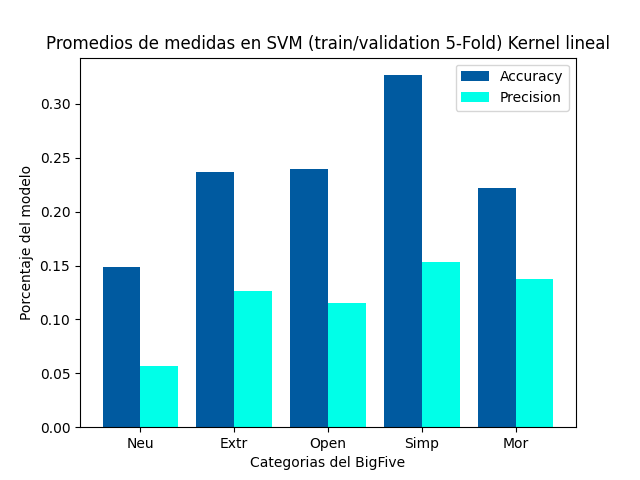
\includegraphics[width = 0.3\linewidth]{Medias_Lineal10.png}
                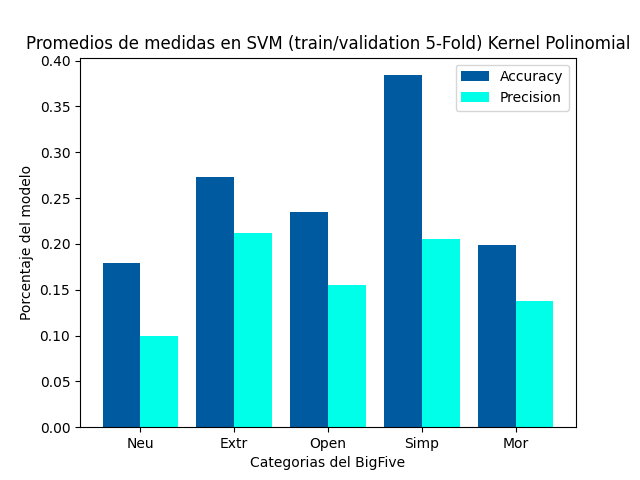
\includegraphics[width = 0.3\linewidth]{Medias_Polinomial10.png}
                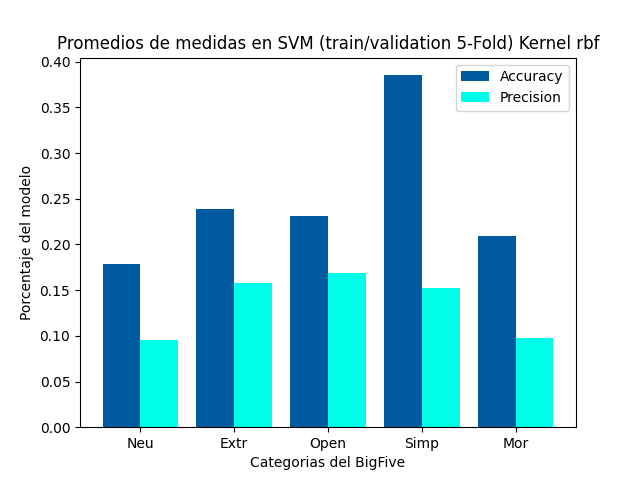
\includegraphics[width = 0.3\linewidth]{Medias_rbf10.png}

            \end{figure}

            Todas por debajo del 50\%, para estos modelos en la etapa de validaci\'on se obtuvieron los 
            siguientes valores de \texttt{accuracy} y las siguientes gr\'aficas para cada kernel. \\ 

            \begin{tabular}[H]{|c|c|c|c|}

                \hline Categor\'ia & Accur (Lineal) & Accur (Polinomial) & Accur (RBF) \\  
                \hline Neuroticismo             & 0.0796 & 0.1401  &  0.1433\\
                \hline Extroversio\'n           & 0.2006 & 0.2101  &  0.2133\\
                \hline Apertura a Exp  & 0.1910 & 0.1942  &  0.1942\\
                \hline Simpat\'ia               & 0.3598 & 0.5350  &  0.4968\\
                \hline Moralidad                & 0.4140 & 0.3789  &  0.3789\\
                \hline
            \end{tabular}

            \begin{figure}[H]
                \centering
                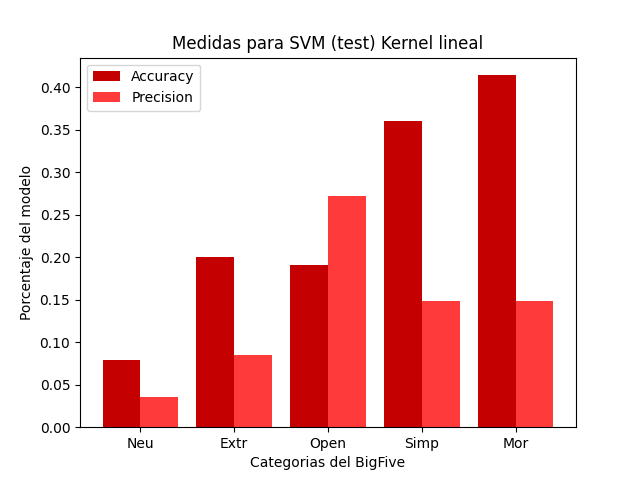
\includegraphics[width = 0.3\linewidth]{final_lineal10.png}
                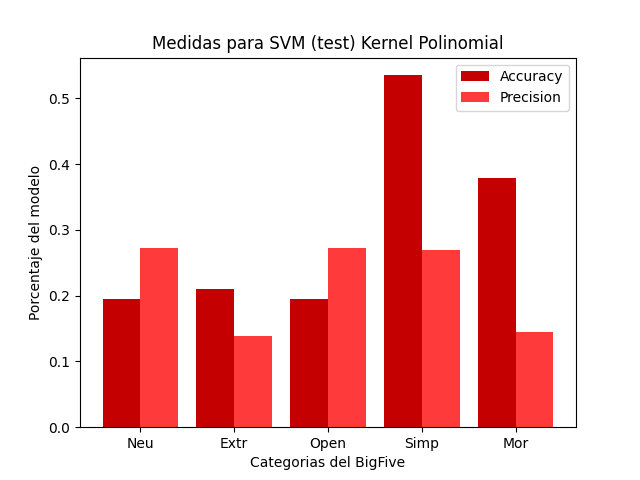
\includegraphics[width = 0.3\linewidth]{final_polinomial10.png}
                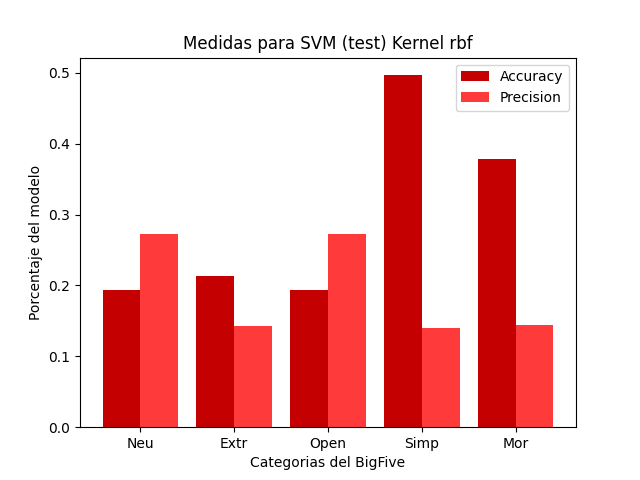
\includegraphics[width = 0.3\linewidth]{final_rbf10.png}

            \end{figure}

            Adem\'as de este enfoque se trat\'o tambi\'en con una clasificaci\'on en dos categor\'ias, Alta( $>~ 80$ ) y Baja( $<= ~80$ ) para
            cada rasgo del BigFive y se obtuvieron resultados que var\'ian entre en 50\% y el 84\% de \texttt{accuracy} en la etapa 
            de entrenamiento/test del modelo tal y como muestran las gr\'aficas:\\ 

            \begin{figure}[H]
                \centering
                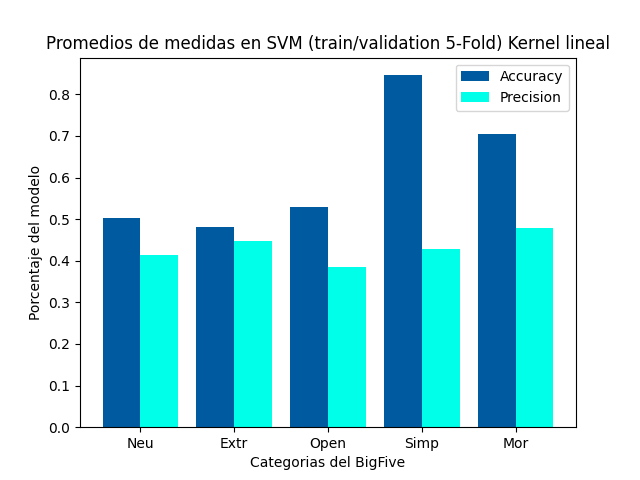
\includegraphics[width = 0.3\linewidth]{Medias_Lineal.png}
                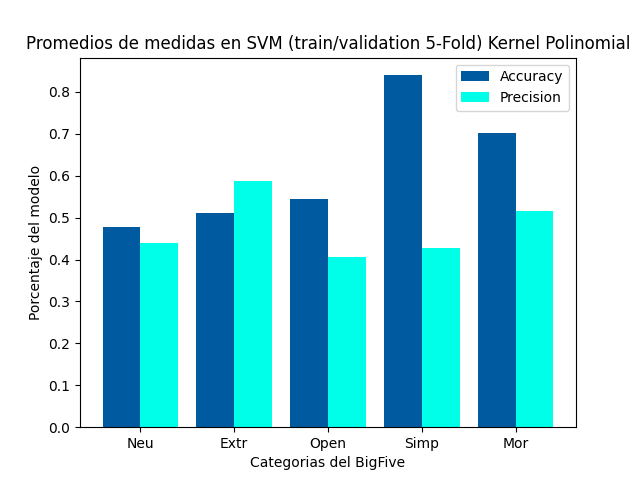
\includegraphics[width = 0.3\linewidth]{Medias_Polinomial.png}
                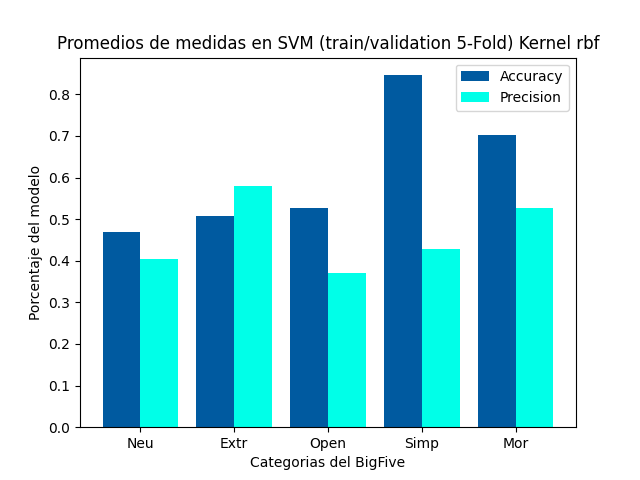
\includegraphics[width = 0.3\linewidth]{Medias_rbf.png}

            \end{figure}

            En la etapa de validaci\'on se obtuvieron los siguientes valores de \texttt{accuracy}: \\ 

            \begin{tabular}[H]{|c|c|c|c|}

                \hline Categor\'ia & Accur (Lineal) & Accur (Polinomial) & Accur (RBF) \\  
                \hline Neuroticismo             & 0.9617 & 0.9171  &  0.9171\\
                \hline Extroversio\'n           & 0.4936 & 0.4681  &  0.4490\\
                \hline Apertura a Exp           & 0.8152 & 0.7898  &  0.7993\\
                \hline Simpat\'ia               & 0.9171 & 0.9171  &  0.9108\\
                \hline Moralidad                & 0.9171 & 0.8885  &  0.9171\\
                \hline
            \end{tabular}

          
            \begin{figure}[H]
                \centering
                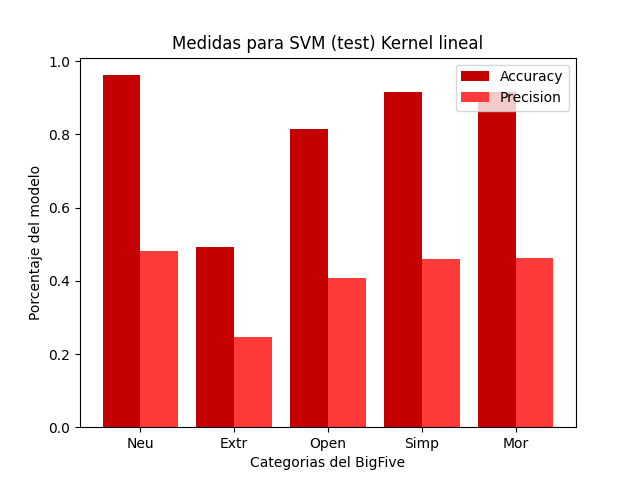
\includegraphics[width = 0.3\linewidth]{final_lineal.png}
                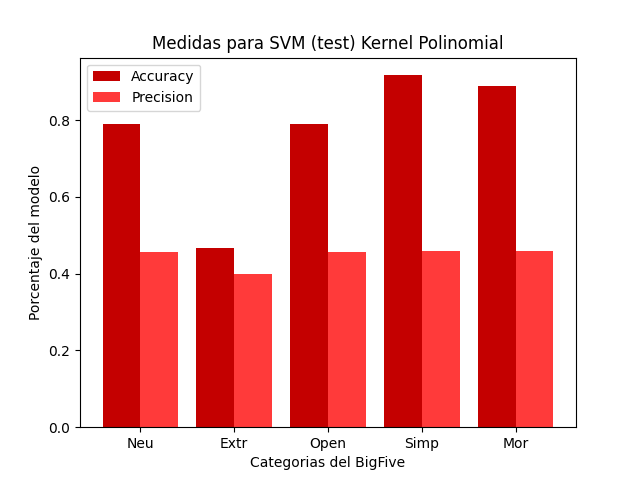
\includegraphics[width = 0.3\linewidth]{final_polinomial.png}
                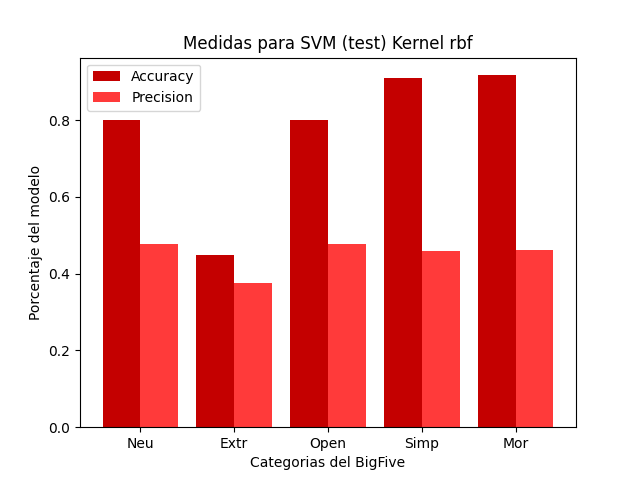
\includegraphics[width = 0.3\linewidth]{final_rbf.png}

            \end{figure}

            Por \'ultimo se trat\'o de predecir en simult\'aneo los 5 rasgos, para ello se tom\'o el vetor binario resultante de 
            clasificar cada categor\'ia como alta o baja t se convirti\'o a decimal, con lo que se tienen $2^5$ grupos posibles, como era de esperar 
            debido a las dimensiones del dataset se obtuvieron bajos resultados para este enfoque debido a underfit, las gr\'aficas de las etapas entrenamiento/test y 
            validaci\'on se muestran a continuaci\'on, igual que los valores de \texttt{accuracy} en la etapa de validaci\'on final para el SVM con cad kernel. 

            \begin{figure}[H]
                \centering
                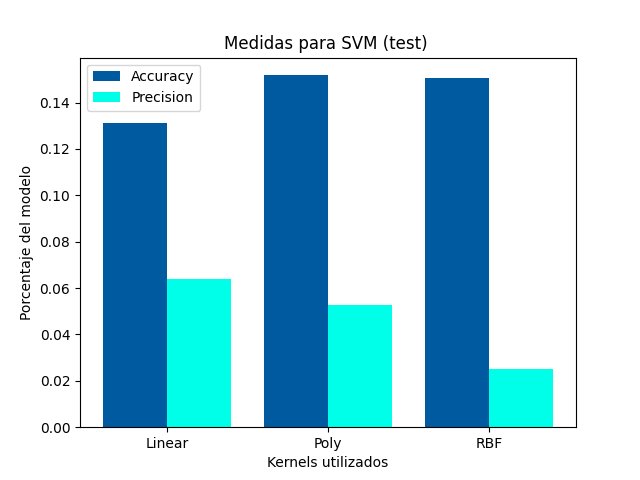
\includegraphics[width = 0.45\linewidth]{Medias_group.png}
                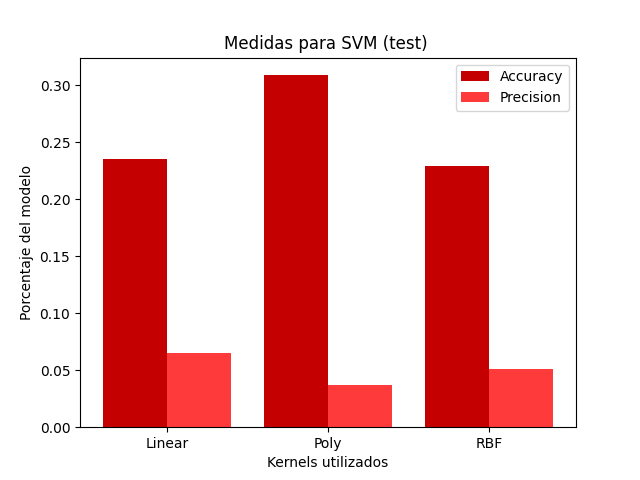
\includegraphics[width = 0.45\linewidth]{final_gruop.png}

            \end{figure}

            \begin{itemize}
                \item [] Accuracy kernel lineal: 0.2365
                \item [] Accuracy kernel polinomial: 0.3089
                \item [] Accuracy kernel rbf: 0.2292
            \end{itemize}
	
		\subsection{K-Means}
		
		El paso inicial para utilizar el m\'etodo KMeans de sklearn es configurar el parámetro \textit{random\_state} el cual determina la generación de números aleatorios para la inicialización del centroide. De esta forma se puede asegurar que los resultados sean consistentes a trav\'es de múltiples ejecuciones. En dependencia de este valor podemos obtener distintos resultados a la hora de agrupar. Se hicieron pruebas para distintos valores de este par\'ametro, algunas de las cuales pueden ser encontradas en el directorio \textit{KMeans\_plots} del repositorio. Finalmente se decidi\'o tomar \textit{random\_seed = 45}.
		
		Luego, se aplican los m\'etodos del codo y la silueta para un rango de cl\'usters determinado, teniendo en cuenta ambos para poder escoger el n\'umero k \'optimo de cl\'usters. Adem\'as se grafican los datos despu\'es de ser agrupados para los mejores k. Se pueden encontrar para cada valor de \textit{random\_seed} todas las gr\'aficas generadas por los m\'etodos anteriores tambi\'en en el directorio \textit{KMeans\_plots}.
		 
		Finalmente, se toman los centroides de cada cl\'uster, 
		se agrupan las caracter\'isticas correspondientes a cada dato seg\'un dichos cl\'usters, y se toma su promedio como representativo del grupo. 
		
		\subsubsection{Descubrir rasgos de caligraf\'ia a partir de rasgos de personalidad}
		
		\begin{figure}[H]
			\centering
			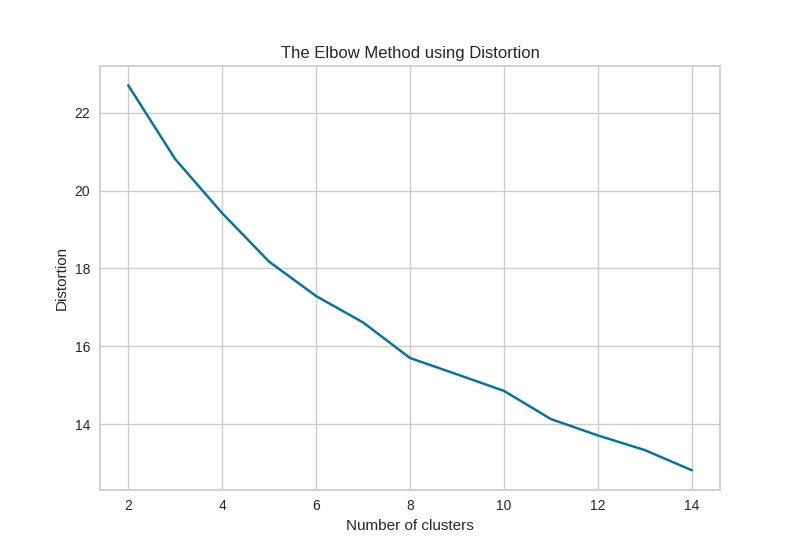
\includegraphics[width = 6cm]{ElbowM_Distortion_bf.png}
			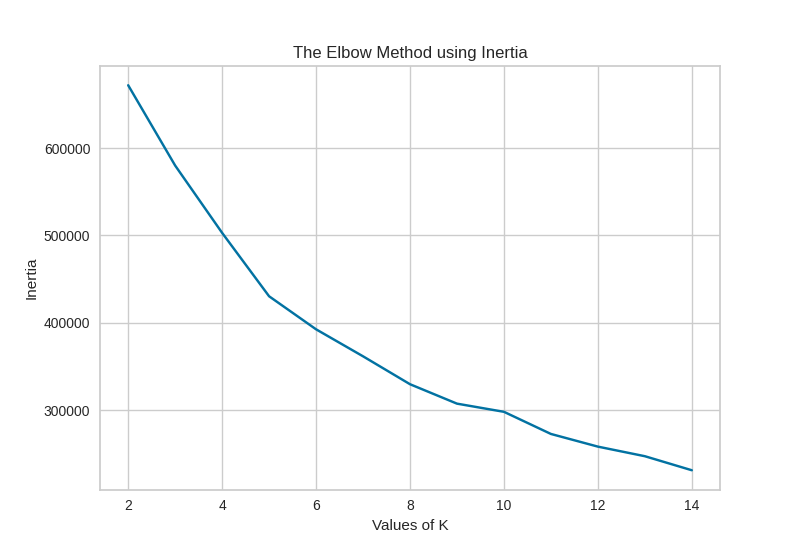
\includegraphics[width = 6cm]{ElbowM_Inertia_bf.png}
			\caption{M\'etodo del codo para medidas distorsi\'on (izquierda) e inercia (derecha) con n\'umero de cl\'usters=[2, 14].}
		\end{figure}
	
		\begin{figure}[H]
			\centering
			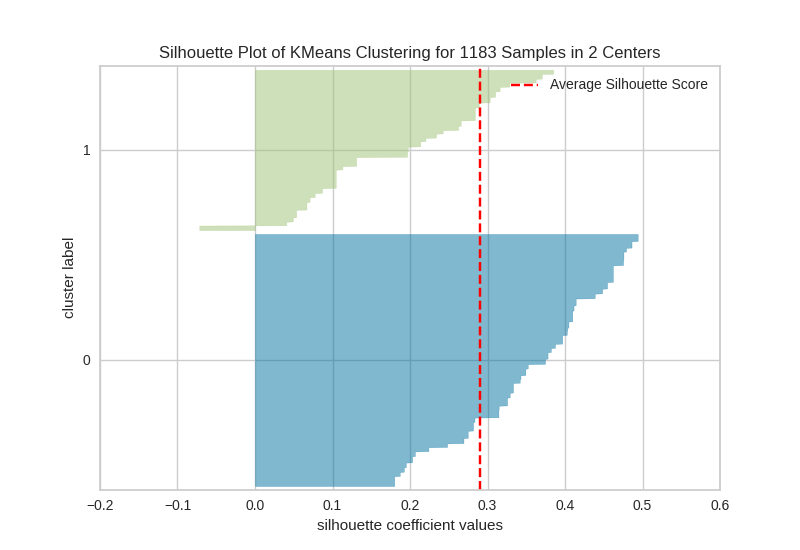
\includegraphics[width = 3.5cm]{silhouette_visualization_2_bf.png}
			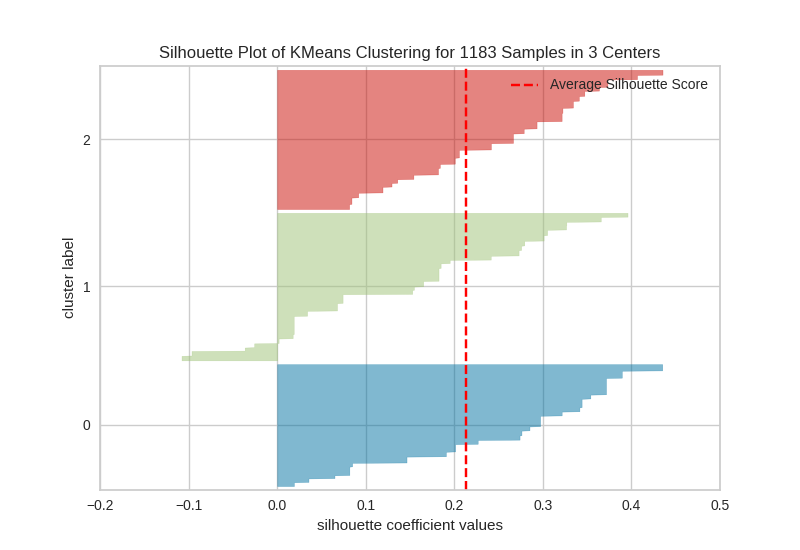
\includegraphics[width = 3.5cm]{silhouette_visualization_3_bf.png}
			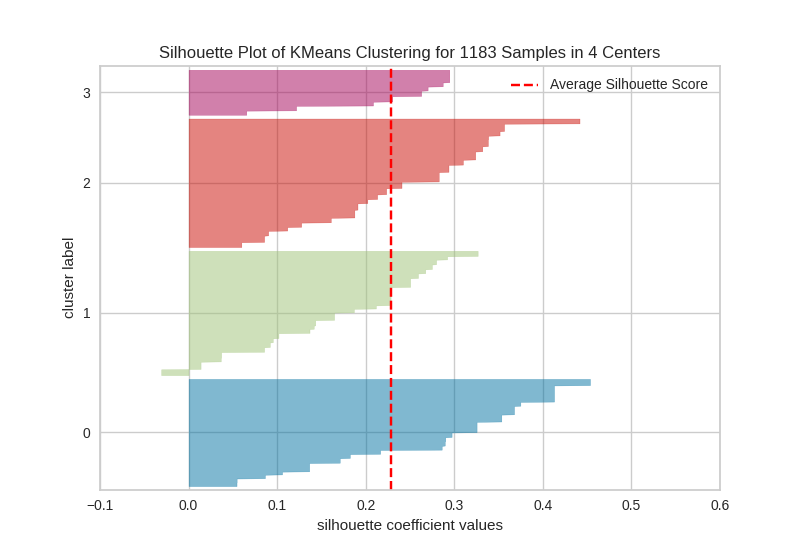
\includegraphics[width = 3.5cm]{silhouette_visualization_4_bf.png}
			
			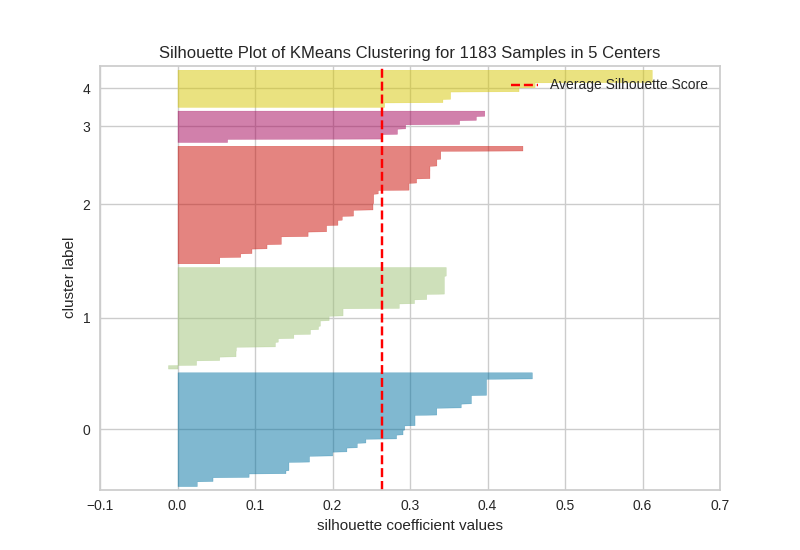
\includegraphics[width = 3.5cm]{silhouette_visualization_5_bf.png}
			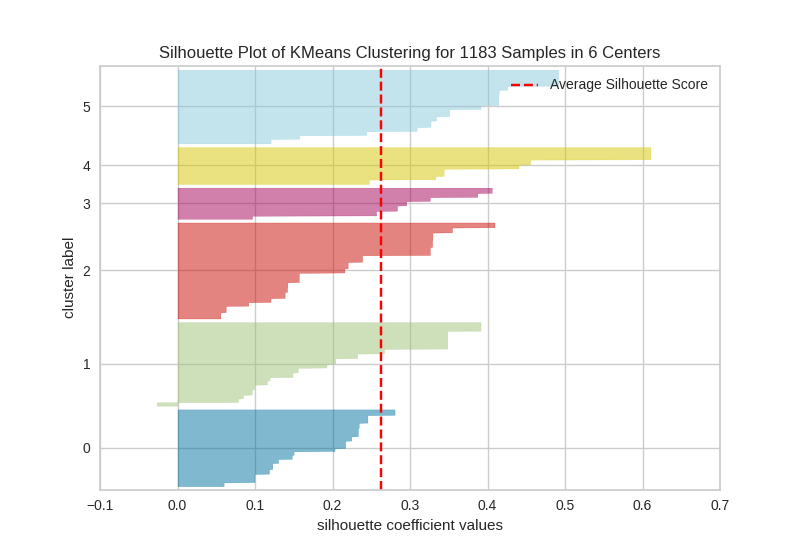
\includegraphics[width = 3.5cm]{silhouette_visualization_6_bf.png}
			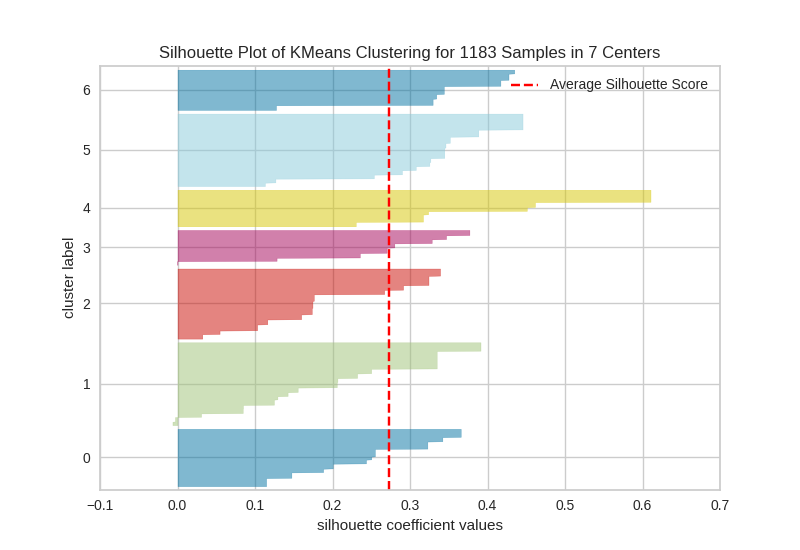
\includegraphics[width = 3.5cm]{silhouette_visualization_7_bf.png}
			
			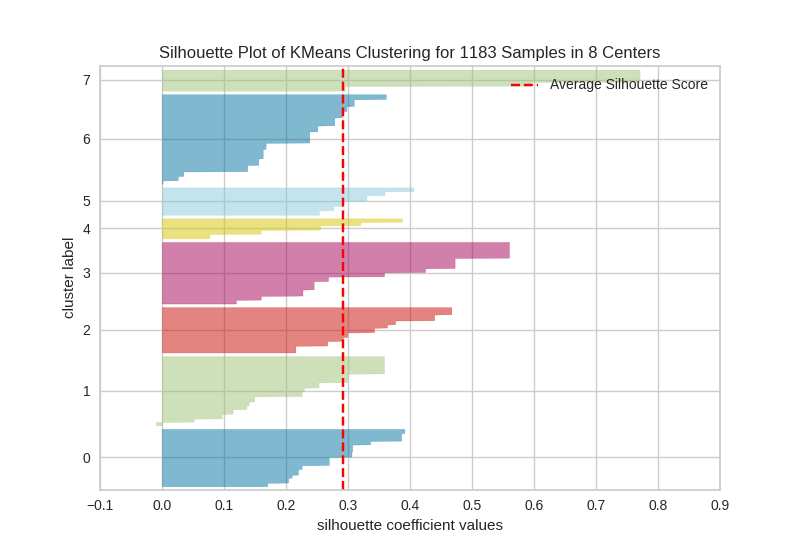
\includegraphics[width = 3.5cm]{silhouette_visualization_8_bf.png}
			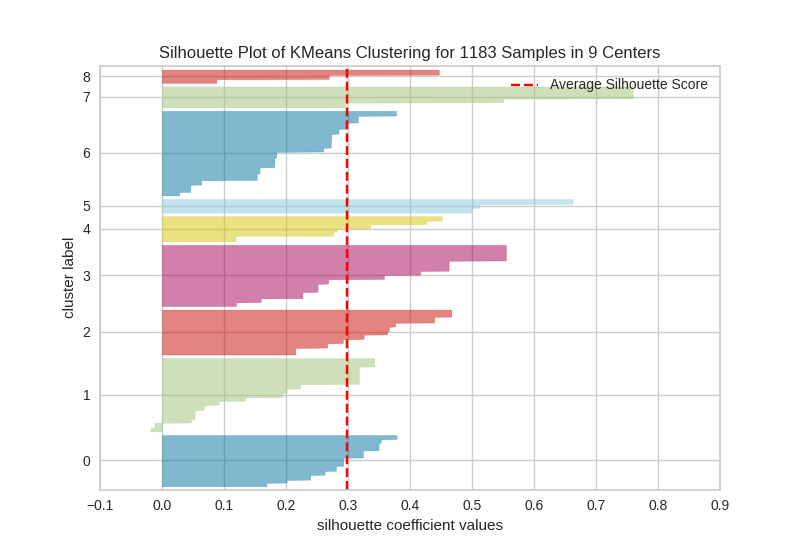
\includegraphics[width = 3.5cm]{silhouette_visualization_9_bf.png}
			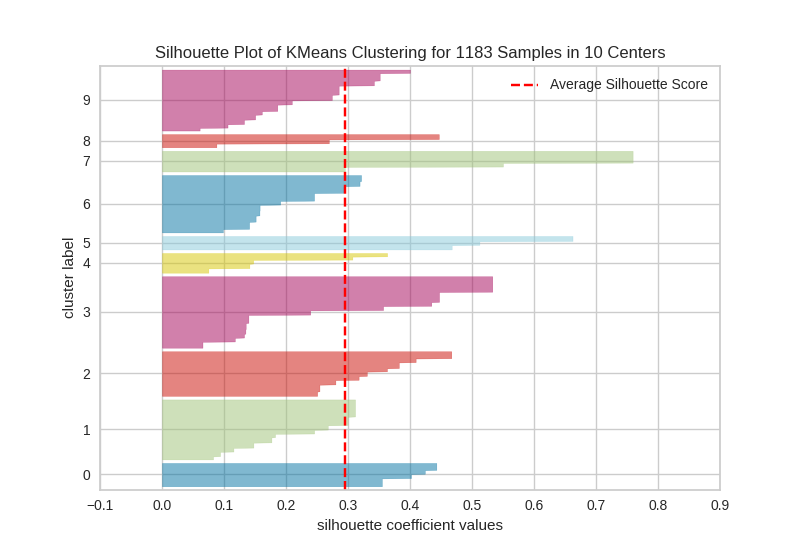
\includegraphics[width = 3.5cm]{silhouette_visualization_10_bf.png}
		
			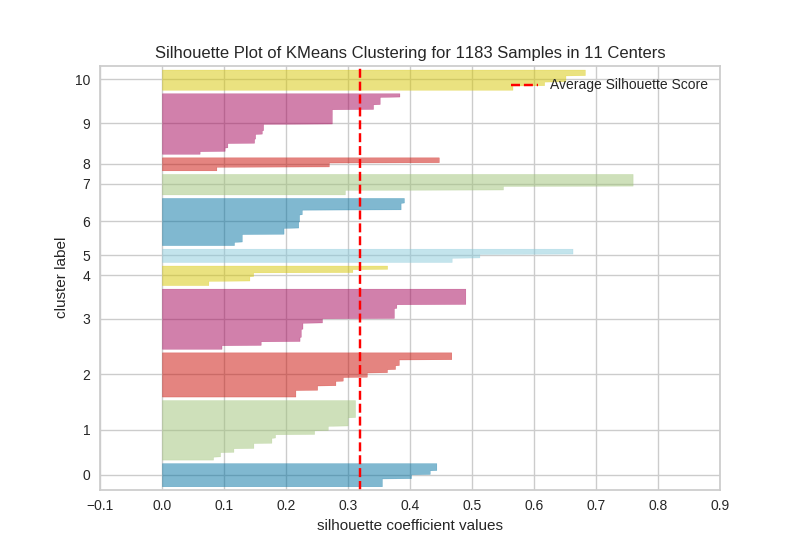
\includegraphics[width = 3.5cm]{silhouette_visualization_11_bf.png}
			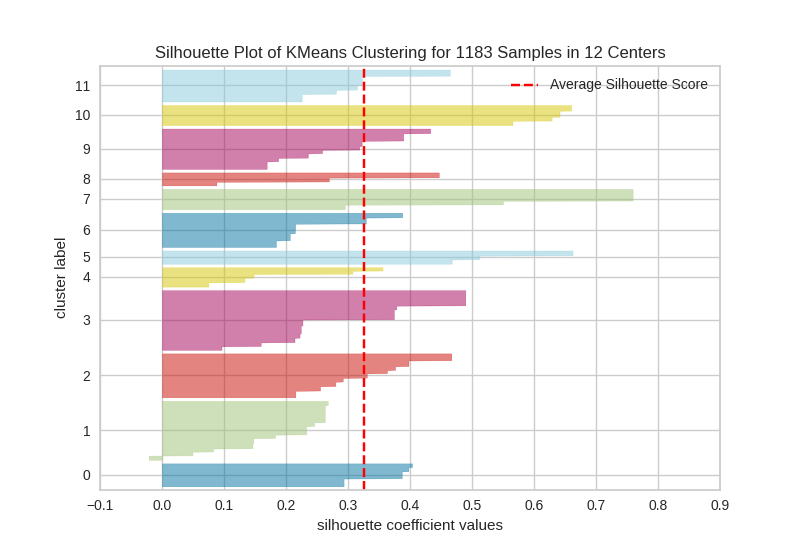
\includegraphics[width = 3.5cm]{silhouette_visualization_12_bf.png}
			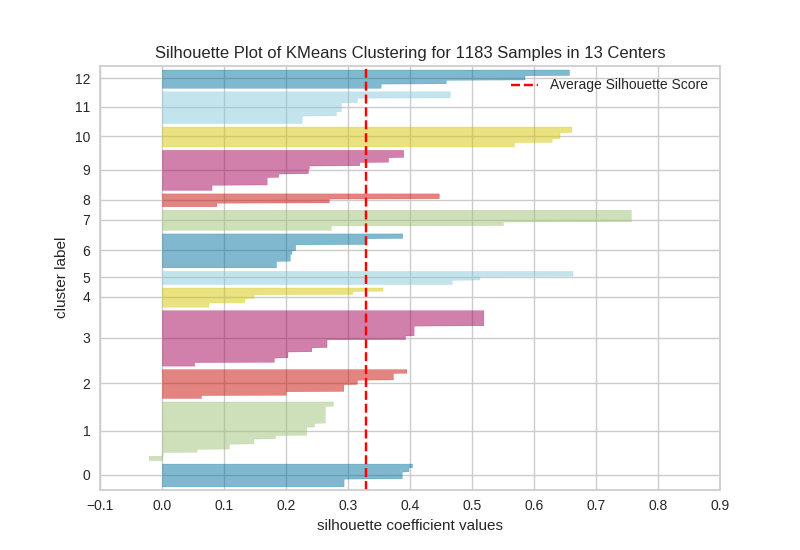
\includegraphics[width = 3.5cm]{silhouette_visualization_13_bf.png}
			
			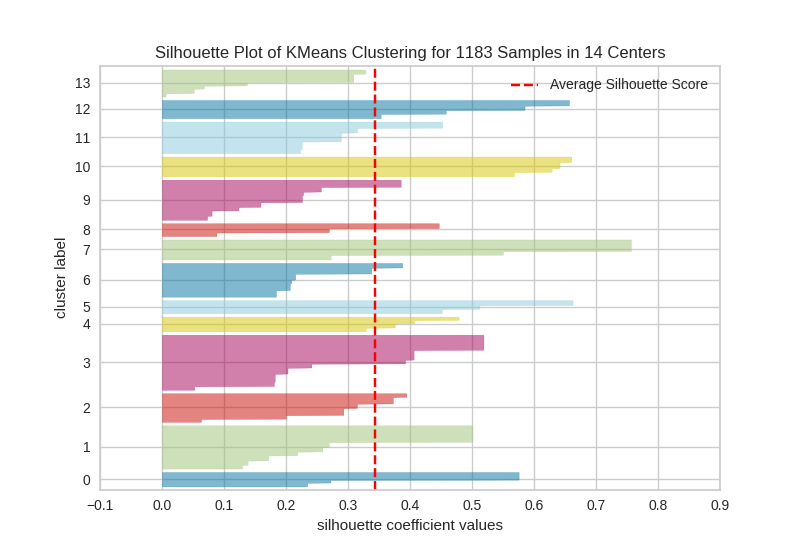
\includegraphics[width = 3.5cm]{silhouette_visualization_14_bf.png}
			
			\caption{M\'etodo de la silueta con n\'umero de cl\'usters=[2, 14].}
		\end{figure}
		
		\begin{figure}[H]
			\centering
			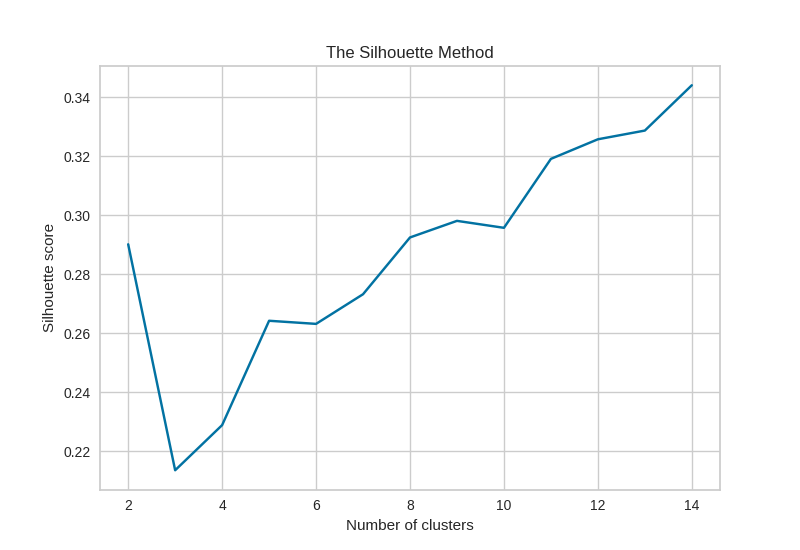
\includegraphics[width = 6cm]{SilhouetteM_bf.png}
			\caption{M\'etodo de la silueta con n\'umero de cl\'usters=[2, 14].}
		\end{figure}
		
		Teniendo en cuenta los resultados mostrados en las gr\'aficas anteriores se determin\'o que el n\'umero \'optimo de cl\'usters es k = 10. 
		
		\begin{figure}[H]
			\centering
			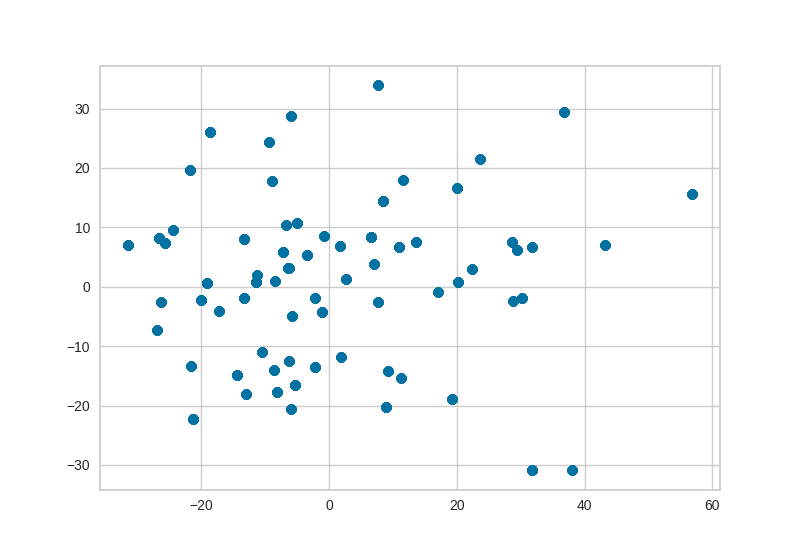
\includegraphics[width = 6cm]{Original_Data_2d_bf.png}
			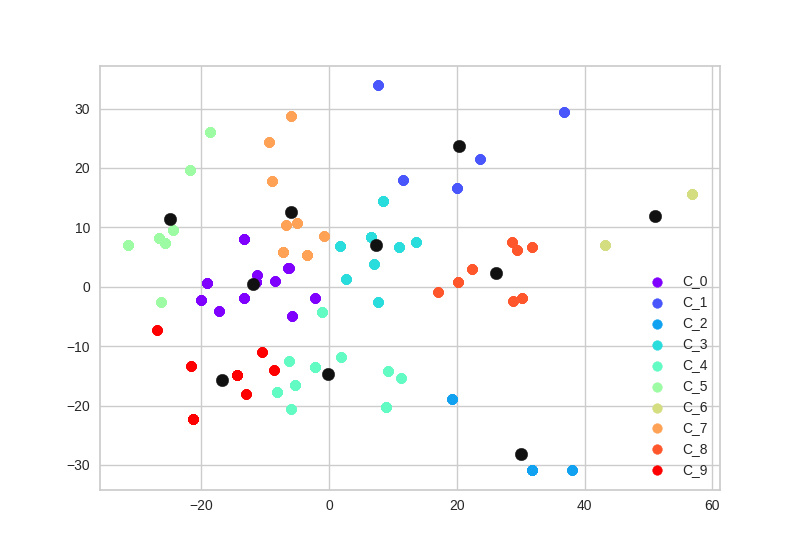
\includegraphics[width = 6cm]{Clustered_Data_2d_k10_seed45_bf.png}
			\caption{Datos originales (izquierda) y datos despu\'es de aplicarles clustering (derecha) para k=10 en dos dimensiones.}
		\end{figure}
		
		\begin{figure}[H]
			\centering
			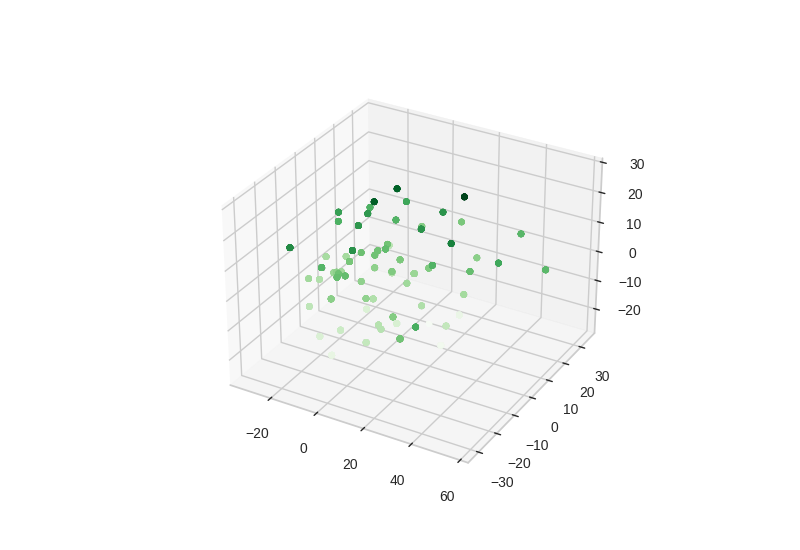
\includegraphics[width = 6cm]{Original_Data_3d_bf.png}
			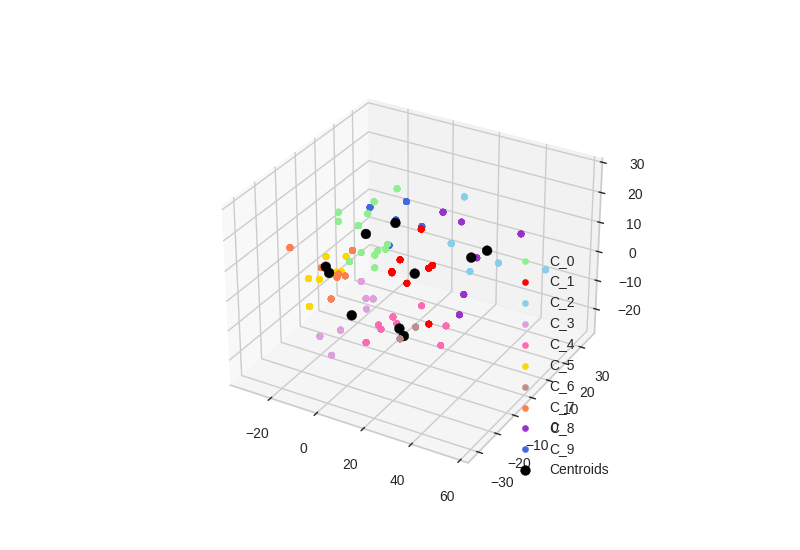
\includegraphics[width = 6cm]{Clustered_Data_3d_k10_seed45_bf.png}
			\caption{Datos originales (izquierda) y datos despu\'es de aplicarles clustering (derecha) para k=10 en tres dimensiones.}
		\end{figure}
		
		Dado al tama\~no del dataset y la poca diversidad de los datos el modelo no es capaz de extraer muchas conclusiones. N\'otese que el vector promedio de features por cl\'uster es igual en todos excepto para el cl\'uster n\'umero 7. De este podemos saber que las personas con baja Moralidad y todos los dem\'as rasgos altos, tienden a escribir con m\'argenes anchos.
		
		\begin{center}
			\begin{tabular}[H]{|c|c|c|}
			\hline Cl\'uster & Promedio Big Five (centroides) & Promedio features \\  
			\hline 0 & 58. 70. 91. 95. 79. & 0. 0. 1. 0. 0. \\
			\hline 1 & 81. 74. 81. 78. 85. & 0. 0.  1.  0.  0. \\
			\hline 2 & 86. 91. 88. 97. 89. & 0. 0.  1.  0.  0. \\
			\hline 3 & 64. 94. 93. 97. 89. & 0.  0.  1.  0.  0.\\
			\hline 4 & 80. 56. 75. 92. 91. & 0. 0. 1. 0. 0.\\
			\hline 5 & 83. 71. 71. 88. 57. & 0. 0.  1.  0.  0.\\
			\hline 6 & 58.  85.  78.  97. 105. & 0. 0. 1. 0. 0.\\
			\hline 7 & 94. 92. 98. 86. 57. & 0. 0.  1.  0.  1.\\
			\hline 8 & 96. 49. 75. 81. 60. & 0. 0.  1.  0.  0. \\
			\hline 9 & 66. 76. 80. 94. 93. & 0.  0.  1.  0.  0.\\
			\hline
		\end{tabular}
		\end{center}
		
		
		\subsubsection{Descubrir rasgos de personalidad a partir de features}
    	
   		\begin{figure}[H]
    		\centering
    		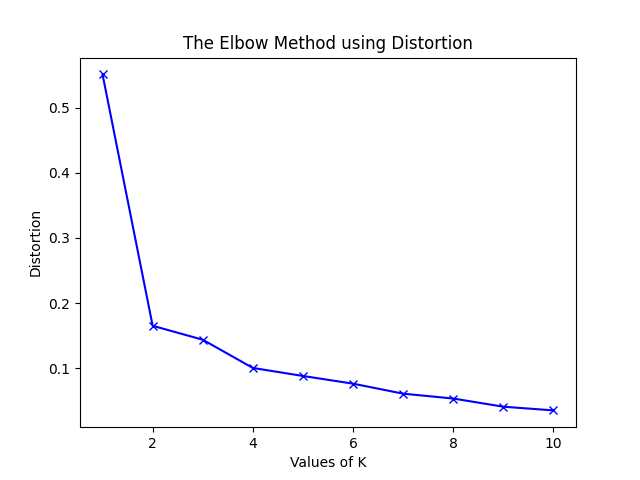
\includegraphics[width = 6cm]{ElbowM_Distortion.png}
    		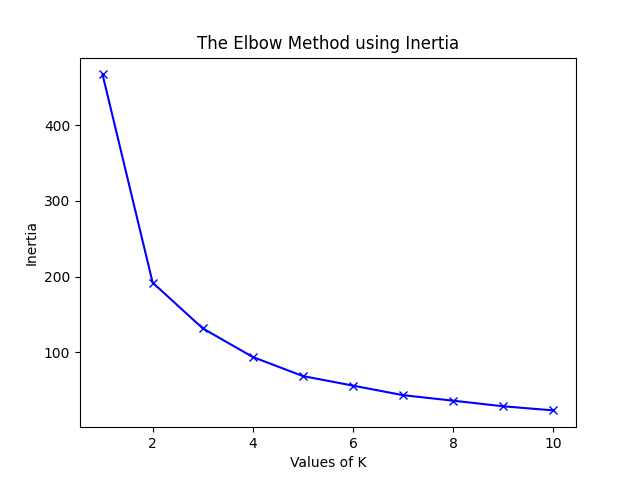
\includegraphics[width = 6cm]{ElbowM_Inertia.png}
    		\caption{M\'etodo del codo para medidas distorsi\'on (izquierda) e inercia (derecha) con n\'umero de cl\'usters=[2, 10].}
    	\end{figure}

    	\begin{figure}[H]
    		\centering
    		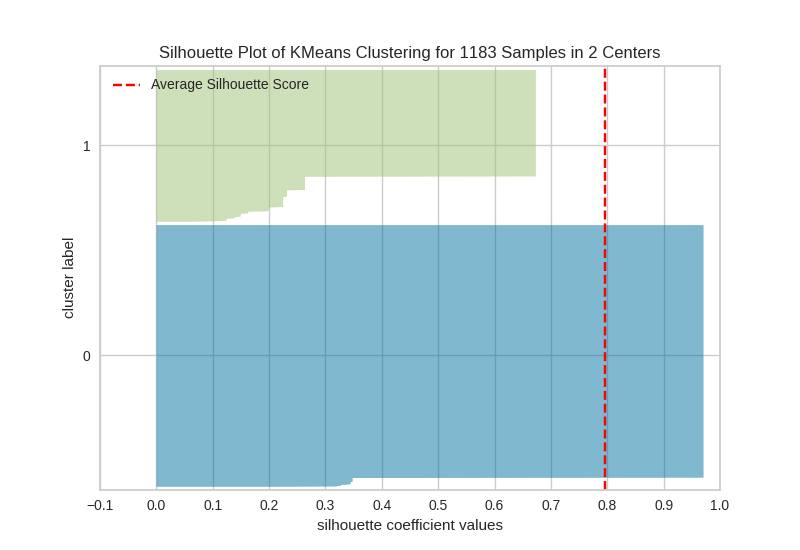
\includegraphics[width = 3.5cm]{silhouette_visualization_2.png}
    		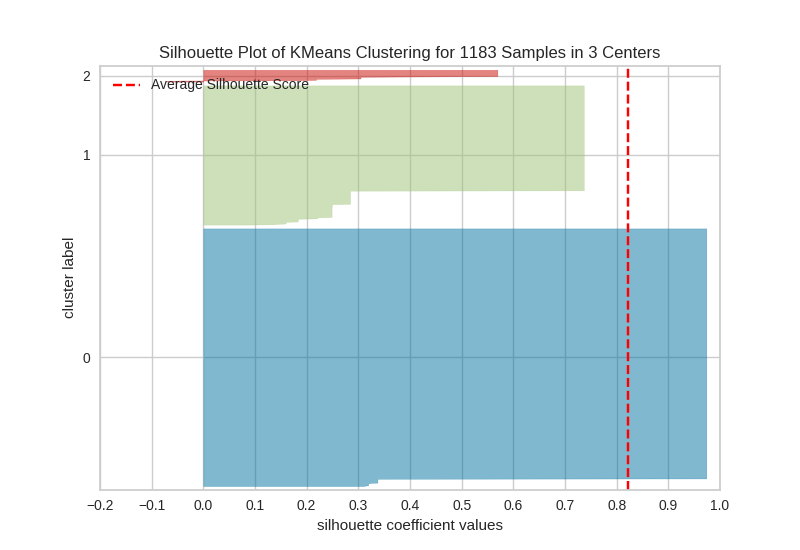
\includegraphics[width = 3.5cm]{silhouette_visualization_3.png}
    		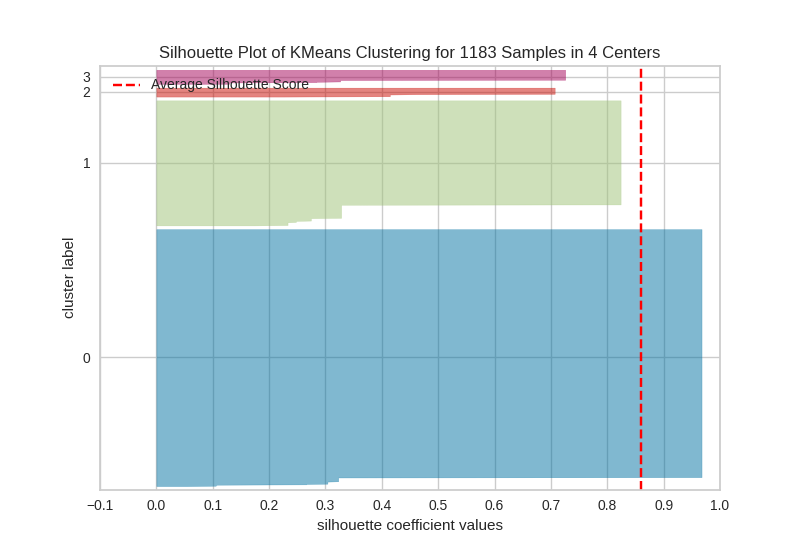
\includegraphics[width = 3.5cm]{silhouette_visualization_4.png}
    		
    		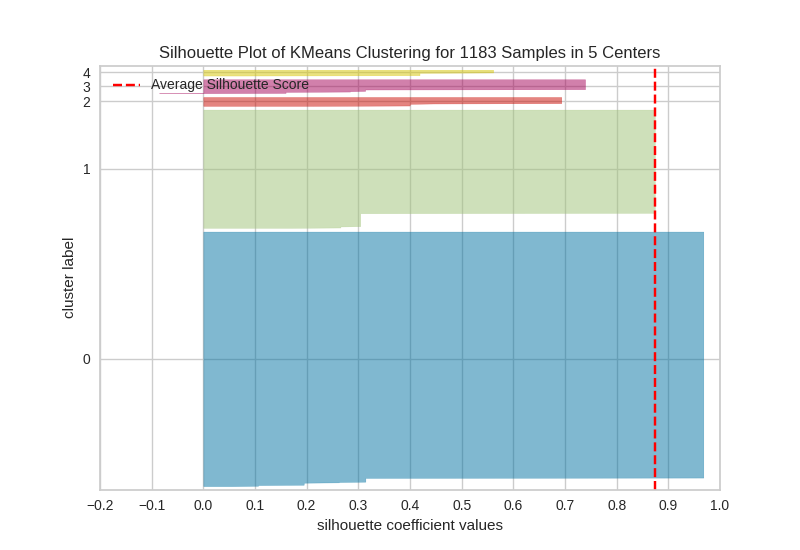
\includegraphics[width = 3.5cm]{silhouette_visualization_5.png}
    		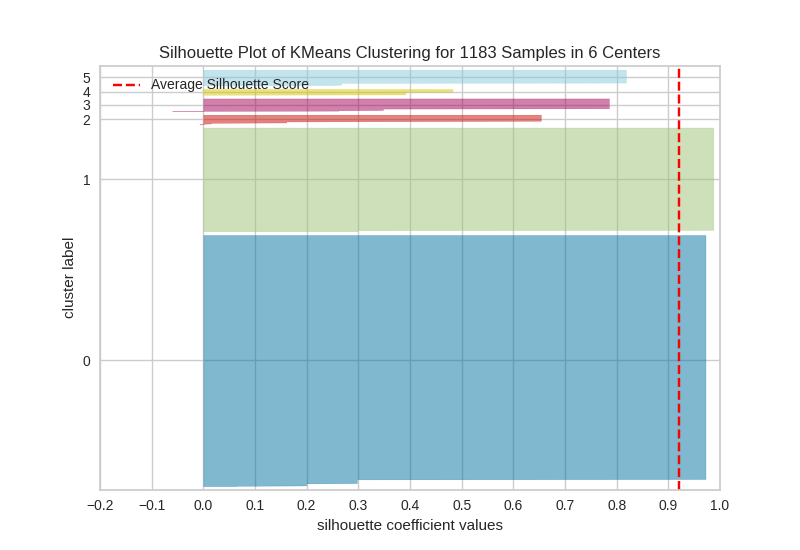
\includegraphics[width = 3.5cm]{silhouette_visualization_6.png}
    		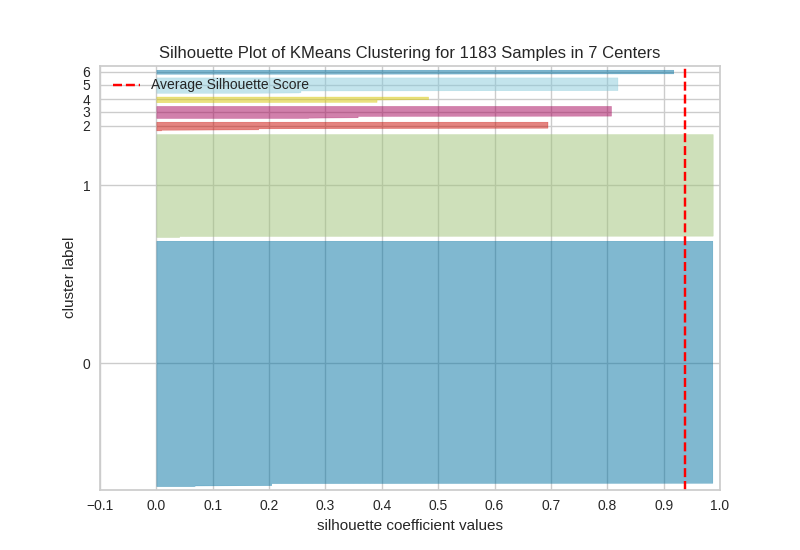
\includegraphics[width = 3.5cm]{silhouette_visualization_7.png}
    		
    		\includegraphics[width = 3.5cm]{silhouette_visualization_8.png}
    		\includegraphics[width = 3.5cm]{silhouette_visualization_9.png}
    		\includegraphics[width = 3.5cm]{silhouette_visualization_10.png}
    		
    		\caption{M\'etodo de la silueta con n\'umero de cl\'usters=[2, 10].}
    	\end{figure}
    	
    	\begin{figure}[H]
    		\centering
    		\includegraphics[width = 6cm]{SilhouetteM.png}
    		\caption{M\'etodo de la silueta con n\'umero de cl\'usters=[2, 10].}
    	\end{figure}
    	
    	Teniendo en cuenta los resultados mostrados en las gr\'aficas anteriores se determin\'o que el n\'umero \'optimo de cl\'usters es k = 7.
    	
    	\begin{figure}[H]
    		\centering
    		\includegraphics[width = 6cm]{Original_Data_2d.png}
    		\includegraphics[width = 6cm]{Clustered_Data_2d_k7_seed45.png}
    		\caption{Datos originales (izquierda) y datos despu\'es de aplicarles clustering (derecha) para k=7 en dos dimensiones.}
    	\end{figure}
    	
    	\begin{figure}[H]
    		\centering
    		\includegraphics[width = 6cm]{Original_Data_3d.png}
    		\includegraphics[width = 6cm]{Clustered_Data_3d_k7_seed45.png}
    		\caption{Datos originales (izquierda) y datos despu\'es de aplicarles clustering (derecha) para k=7 en tres dimensiones.}
    	\end{figure}
    	
    	\begin{tabular}[H]{|c|c|c|}
    		\hline Cl\'uster & Promedio features (centroides) & Promedio Big Five  \\  
    		\hline 0 & 0. 0.  1.  0. 0. & 73. 79. 84. 92. 87. \\
    		\hline 1 & 0.  0.  1.  0.  1. & 69. 83. 84. 92. 88.\\
    		\hline 2 &  1.  0.  1. 0.  1. & 75. 81. 83. 92. 85. \\
    		\hline 3 & 0. 1. 1. 0. 1. & 74. 81. 83. 87. 90. \\
    		\hline 4 & 1. 0.  1.  0.  1. & 74. 84. 84. 91. 87. \\
    		\hline 5 &  0. -1. 1.  0.  1. & 78. 81. 85. 87. 79. \\
    		\hline 6 & 0. 0. 1.  1. 0. & 80. 74. 82. 96. 83. \\
    		\hline
    	\end{tabular}
    
    
   
    
   
   
    
    \section{Conclusiones y trabajo futuro}
        En este trabajo se realiz\'o un estudio profundo de aprendizaje de m\'aquinas aplicado a Grafolog\'ia, desde la consulta al Estado del Arte, Construcci\'on y Taggeo de un Dataset, extracci\'on de Features de las im\'agenes, entrenamiento de algoritmos y an\'alisis de resultados. A modo general el flujo de trabajo queda representado en la siguiente imagen: 

        \begin{figure}[H]
            \centering
            \includegraphics[width = 0.5\linewidth]{photo_2023-05-29_02-40-00.jpg}
            \caption{Flujo del trabajo del Proyecto.}
        \end{figure}

        Con los algoritmos empleados pudimos concluir que realmente la grafolog\'ia no puede determinar de 
        forma certera la psicolog\'ia de una persona. Los modelos utilizados rondan el 50\% de efectividad en sus predicciones, lo cual dista de ser una clasificaci\'on fiable. De los modelos utilizados el SVM con clasificaciones en alto y bajo es el que mejores 
        resultados ofreci\'o, en su mayor\'ia sobre el 80\% - 90\% de fiabilidad, pero igual distante en identificar caracter\'isticas como la extroversi\'on.\\ 

        Se propone como idea de investigaci\'on futura la construcci\'on de un dataset de mayores dimensiones para probar estas y otras ideas de aprendizaje de m\'aquinas sobre grafolog\'ia, que permitan que los modelos no hagan overfit por la escas\'es de datos respecto al amplio n\'umero de categor\'ias para clasificar. 

\begin{thebibliography}{99}
    %-----------------------------------------------------------------------------------
        \bibitem{1} \emph{International Conference on Computational Techniques, Electronics and Mechanical.} 2018. 
    
        \bibitem{2} \emph{Handwriting Analysis based on Histogram of Oriented Gradient for Predicting Personality traits using SVM.} Procedia Computer Science, vol. 165, 2019.
    
        \bibitem{3} \emph{Personality Prediction based on Handwriting using Machine Learning.}
        
        \bibitem{4} \emph{A framework for analyzing financial behavior using machine learning classification of personality through handwriting analysis.}
    
        \bibitem{5} \emph{E-Graphologist for Personality Profile.}

        \bibitem{6}  \emph{Personality Prediction System Based on Signatures}
        
        \bibitem{7}  \emph{Graphology for Farsi Handwriting Using Image Processing Techniques    }
        
        \bibitem{8}  \emph{A Framework for Determining the Big Five Personality Traits Using Machine Learning Classification through Graphology}
        
        \bibitem{9}  \emph{Personality analysis through handwriting recognition}
        
        \bibitem{10} \emph{Personality Type Assessment System by using  Enneagram-Graphology Techniques on Digital  Handwriting}
        
        \bibitem{11} \emph{Analysis of Signature for the Prediction of Personality\_Traits}
        
        \bibitem{12} \emph{Artificial Neural Network for Human Behavior Prediction  through Handwriting Analysis}
        
        \bibitem{13} \emph{EMOTHAW\_A\_novel\_database\_for\_emotional\_state\_recog}
        
        \bibitem{14} \emph{IEEE Xplore Full-Text PDF}
        
        \bibitem{15} \url{https://data.csafe.iastate.edu/DataPortal/#HandwritingDatabase} 
        
        \bibitem{16} \url{https://fki.tic.heia-fr.ch/databases/iam-handwriting-database} 

        \bibitem{17} \emph{Forensic Graphology Assessment of Personality}

        \bibitem{18} \emph{Handwriting Personality Recognition with Machine  Learning: A Comparative Study}

        \bibitem{19} \emph{GRAPHOLOGY: UNDERSTANDING – MISUNDERSTANDING.}

        \bibitem{20} \emph{Predicting the Big Five personality traits from handwriting } 2018

        \bibitem{21} \emph{A Machine Learning Approach to Employability Evaluation Using Handwriting Analysis}

        \bibitem{22} \emph{Handwritten document image segmentation into text lines and words} 2010
        
        \bibitem{23} \url{https://bigfive-test.com}
        %-----------------------------------------------------------------------------------
    \end{thebibliography}
\end{document}